% Request path of a cache hit with centralized block discovery (Mooncake-style).
% Build: lualatex request_path.tex   (system Helvetica via fontspec)
\documentclass{article}
\usepackage{fontspec}
\setsansfont{Helvetica}
\renewcommand{\familydefault}{\sfdefault}
\usepackage{tikz}
\usetikzlibrary{arrows.meta,calc}
\pagestyle{empty}

\definecolor{rpc}{HTML}{B2182B}   % metadata RPCs
\definecolor{data}{HTML}{2166AC}  % KV data
\definecolor{nodefill}{gray}{0.94}
\definecolor{subtext}{gray}{0.35}

\tikzset{
  nodebox/.style={draw=black, line width=0.6pt, rounded corners=2pt, fill=nodefill},
  stack/.style={draw=black!55, line width=0.5pt, rounded corners=2pt, fill=nodefill!50!white},
  comp/.style={draw=black, line width=0.5pt, rounded corners=1.5pt, fill=white,
               align=center, inner sep=2pt},
  ttl/.style={font=\footnotesize\bfseries},
  sub/.style={font=\scriptsize, text=subtext},
  step/.style={circle, fill=#1, text=white, font=\fontsize{6}{6}\selectfont\bfseries,
               inner sep=0pt, minimum size=9pt},
  rpcline/.style={{Stealth[length=4.5pt,width=3.8pt]}-{Stealth[length=4.5pt,width=3.8pt]},
                  line width=0.9pt, draw=rpc},
  dataline/.style={-{Stealth[length=6pt,width=5.5pt]}, line width=1.6pt, draw=data},
  blk/.style={draw=black!45, line width=0.4pt, fill=white, minimum size=0.26cm, inner sep=0pt},
}

\begin{document}
\setbox0=\hbox{%
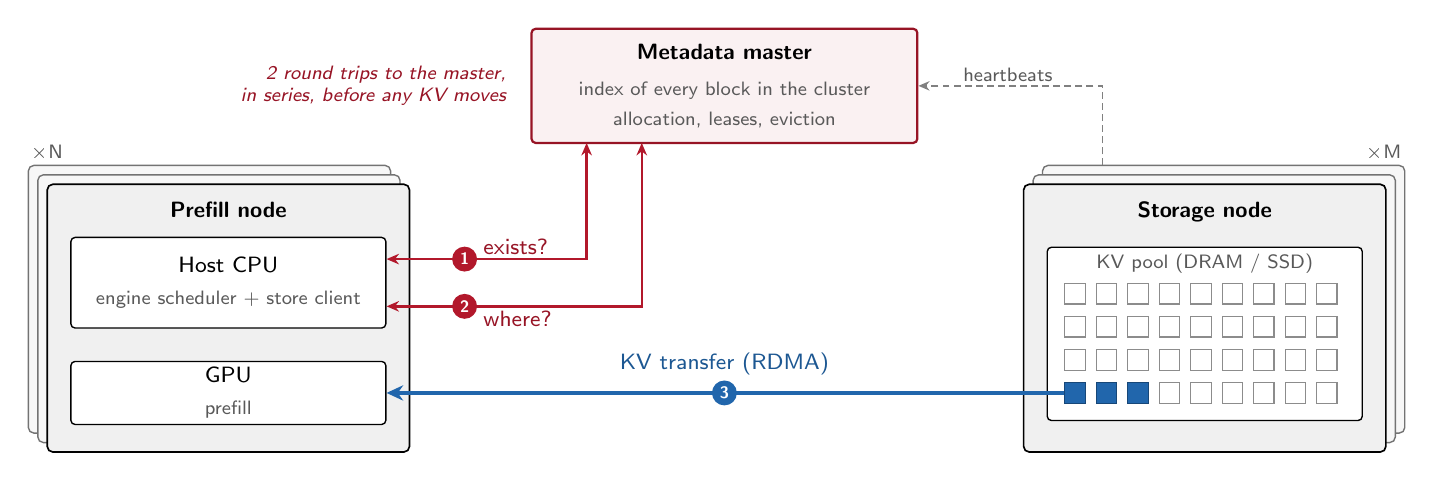
\begin{tikzpicture}[x=1cm,y=1cm]

  % --- Prefill nodes (requesters), drawn as a stack ---------------------------
  \draw[stack] (-0.24,0.24) rectangle ++(4.6,3.4);
  \draw[stack] (-0.12,0.12) rectangle ++(4.6,3.4);
  \draw[nodebox] (0,0) rectangle (4.6,3.4);
  \node[ttl, anchor=north] at (2.3,3.3) {Prefill node};
  \node[sub, anchor=south west, inner sep=1pt] at (-0.24,3.66) {×N};
  \node[comp, minimum width=4.0cm, minimum height=1.15cm] (cpu) at (2.3,2.15)
    {\footnotesize Host CPU\\[-0.5pt]{\scriptsize\color{subtext}engine scheduler + store client}};
  \node[comp, minimum width=4.0cm, minimum height=0.8cm] (gpu) at (2.3,0.75)
    {\footnotesize GPU\\[-0.5pt]{\scriptsize\color{subtext}prefill}};

  % --- Central metadata master ---------------------------------------------
  \node[comp, draw=rpc!85!black, fill=rpc!6, line width=0.8pt,
        minimum width=4.9cm, minimum height=1.45cm] (master) at (8.6,4.65)
    {\footnotesize\bfseries Metadata master\\[1pt]
     {\scriptsize\color{subtext}index of every block in the cluster}\\[-1pt]
     {\scriptsize\color{subtext}allocation, leases, eviction}};
  \node[font=\scriptsize\itshape, text=rpc!85!black, anchor=east, align=right]
    at (5.95,4.65) {2 round trips to the master,\\in series, before any KV moves};

  % --- Storage nodes (owners), drawn as a stack -----------------------------
  \draw[stack] (12.64,0.24) rectangle ++(4.6,3.4);
  \draw[stack] (12.52,0.12) rectangle ++(4.6,3.4);
  \draw[nodebox] (12.4,0) rectangle (17.0,3.4);
  \node[ttl, anchor=north] at (14.7,3.3) {Storage node};
  \node[sub, anchor=south east, inner sep=1pt] at (17.24,3.66) {×M};
  \node[comp, minimum width=4.0cm, minimum height=2.2cm] (pool) at (14.7,1.5) {};
  \node[sub, anchor=north, inner sep=2.5pt] at (pool.north) {KV pool (DRAM / SSD)};
  \foreach \r in {0.75,1.17,1.59,2.01} {
    \foreach \c in {0,...,8} {
      \node[blk] at (13.05+\c*0.4,\r) {};
    }
  }
  \foreach \c in {0,1,2} {
    \node[blk, fill=data, draw=data!70!black] (b\c) at (13.05+\c*0.4,0.75) {};
  }

  % --- Storage nodes register with and heartbeat to the master (off the critical path)
  \draw[-{Stealth[length=4pt,width=3.4pt]}, line width=0.6pt, draw=black!50, dash pattern=on 2.5pt off 1.5pt]
    (13.4,3.64) -- (13.4,4.65) -- (master.east);
  \node[sub, anchor=south, inner sep=1.5pt] at (12.2,4.65) {heartbeats};

  % --- (1) existence check and (2) replica lookup: metadata RPCs ---------------
  \draw[rpcline] (cpu.east |- 0,2.45) -- (6.85,2.45) -- (6.85,3.925);
  \draw[rpcline] (cpu.east |- 0,1.85) -- (7.55,1.85) -- (7.55,3.925);
  \node[step=rpc] at (5.3,2.45) {1};
  \node[step=rpc] at (5.3,1.85) {2};
  \node[font=\footnotesize, text=rpc!85!black, anchor=south west, inner sep=1.5pt]
    at (5.48,2.45) {exists?};
  \node[font=\footnotesize, text=rpc!85!black, anchor=north west, inner sep=1.5pt]
    at (5.48,1.85) {where?};

  % --- (3) KV transfer from the owner ----------------------------------------
  \draw[dataline] (b0.west) -- (gpu.east |- b0.west);
  \node[step=data] at (8.6,0.75) {3};
  \node[font=\footnotesize, text=data!85!black, anchor=south, inner sep=1.5pt]
    at (8.6,0.92) {KV transfer (RDMA)};

\end{tikzpicture}}%
\pdfvariable horigin=0pt
\pdfvariable vorigin=0pt
\pagewidth=\dimexpr\wd0+8pt\relax
\pageheight=\dimexpr\ht0+\dp0+8pt\relax
\shipout\vbox{\kern4pt\hbox{\kern4pt\box0\kern4pt}\kern4pt}
\end{document}
